\subsection*{(c)}
%
Værdien gamma forøger hvor hurtigt befolkningen bliver immun uden at have været smittet. Jo højere værdi af gamma jo hurtigere bliver befolkningen immun, og det maksimale antal der er smittet på en gang falder også. Det kan ses på figurene at hvis gamma ikke er nul så er antallet der bliver inficeret lavere


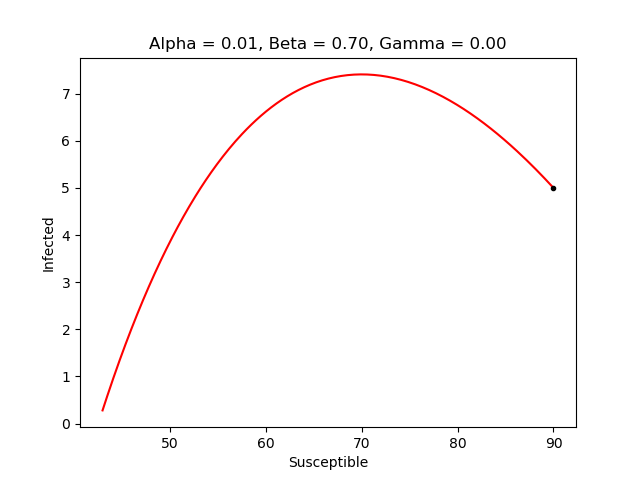
\includegraphics[scale=0.4]{fig/img/a1_b7_g0.png}
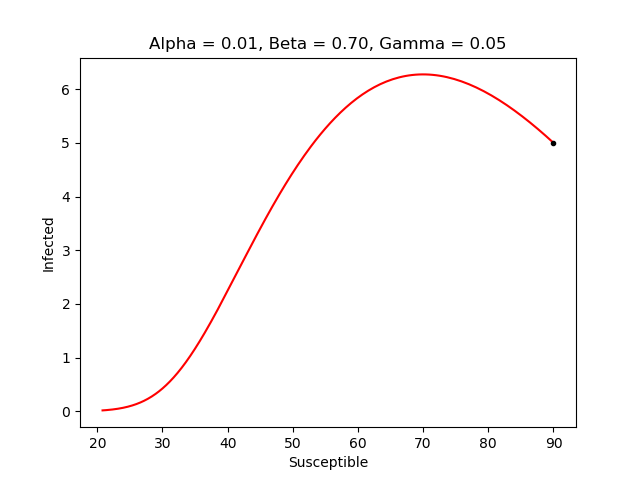
\includegraphics[scale=0.4]{fig/img/a1_b7_g5.png}\\
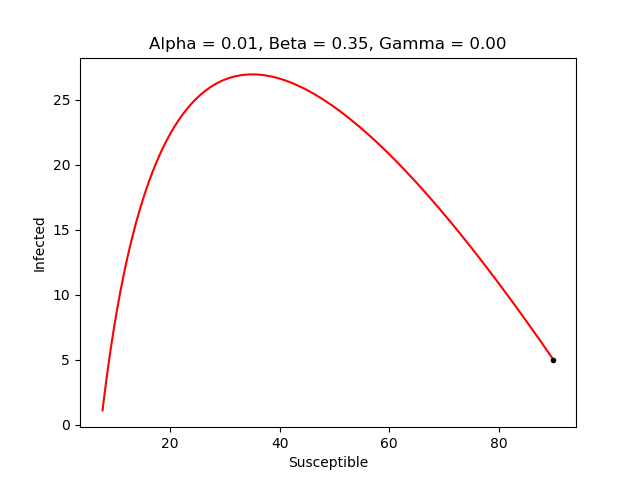
\includegraphics[scale=0.4]{fig/img/a1_b35_g0.png}
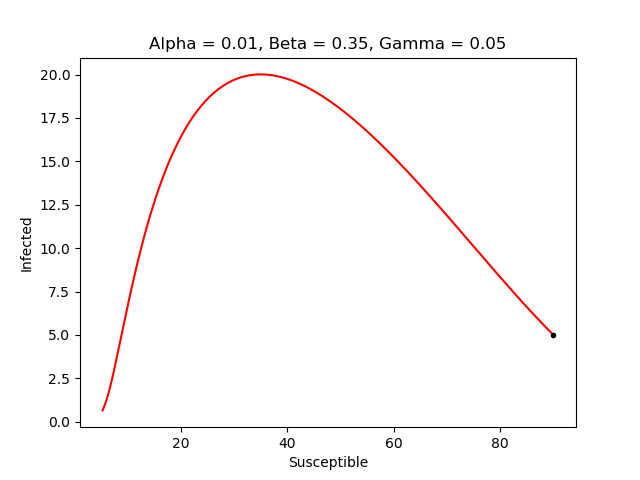
\includegraphics[scale=0.4]{fig/img/a1_b35_g5.png}\\
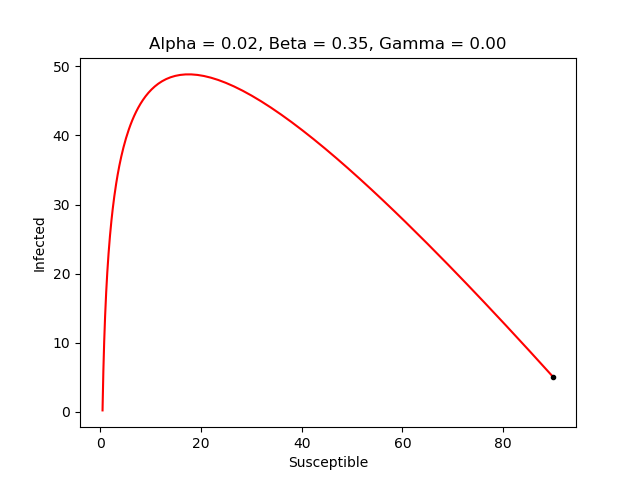
\includegraphics[scale=0.4]{fig/img/a2_b35_g0.png}
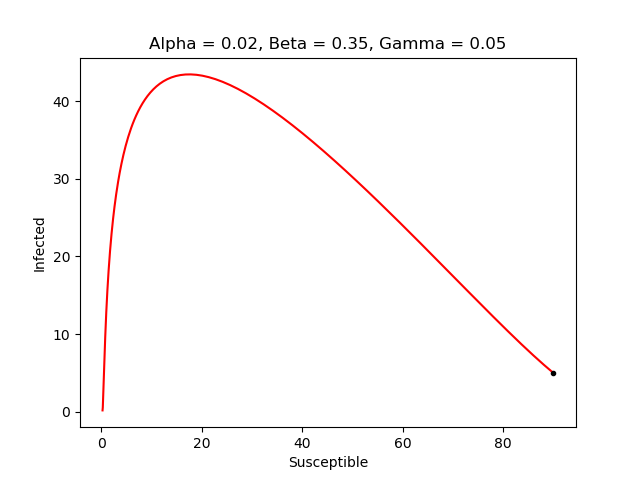
\includegraphics[scale=0.4]{fig/img/a2_b35_g5.png}\\
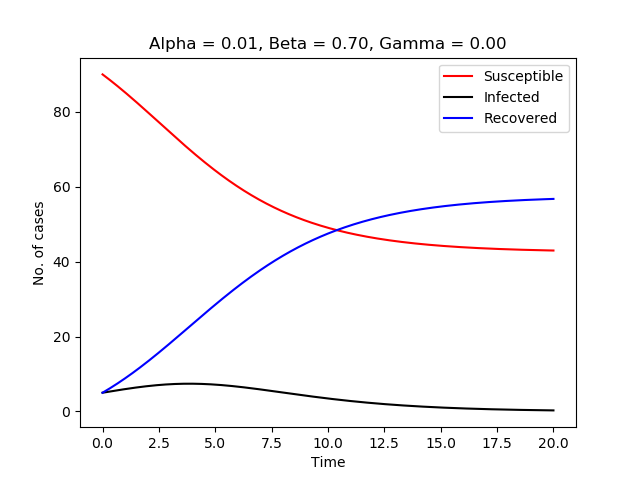
\includegraphics[scale=0.4]{fig/img/t_a1_b7_g0.png}
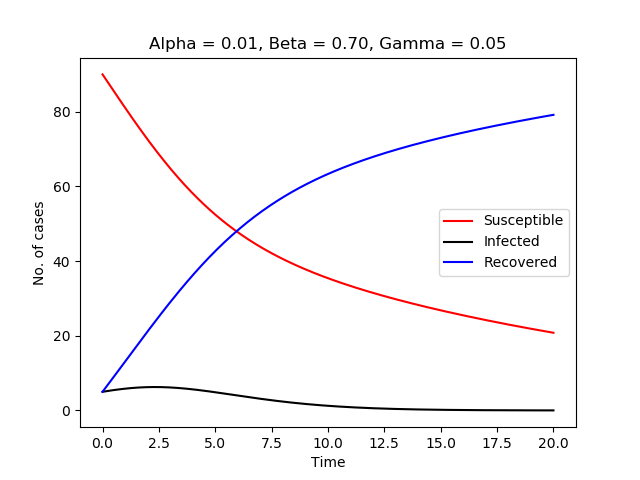
\includegraphics[scale=0.4]{fig/img/t_a1_b7_g5.png}\\
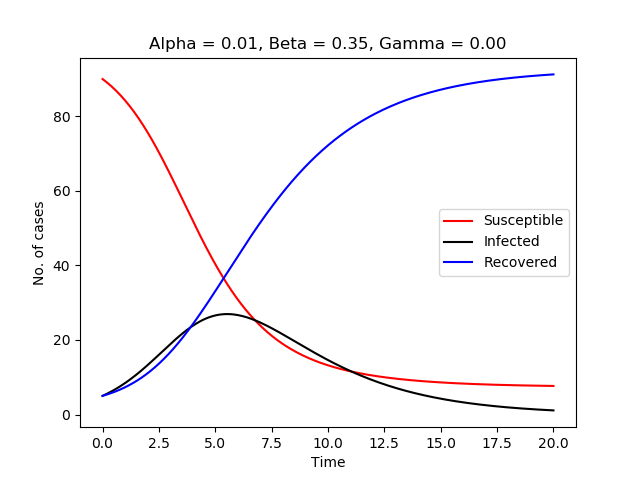
\includegraphics[scale=0.4]{fig/img/t_a1_b35_g0.png}
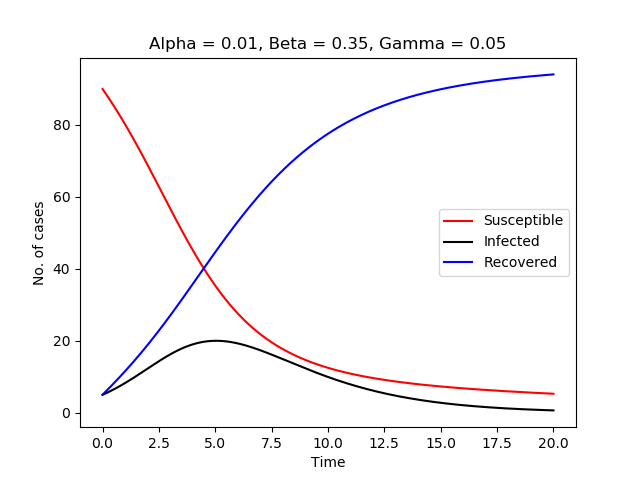
\includegraphics[scale=0.4]{fig/img/t_a1_b35_g5.png}\\
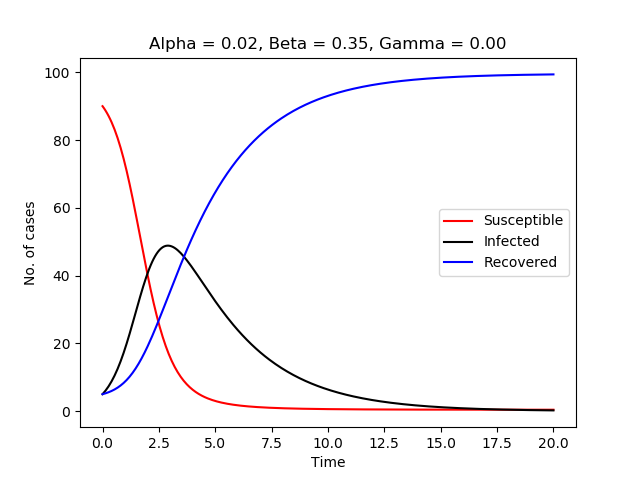
\includegraphics[scale=0.4]{fig/img/t_a2_b35_g0.png}
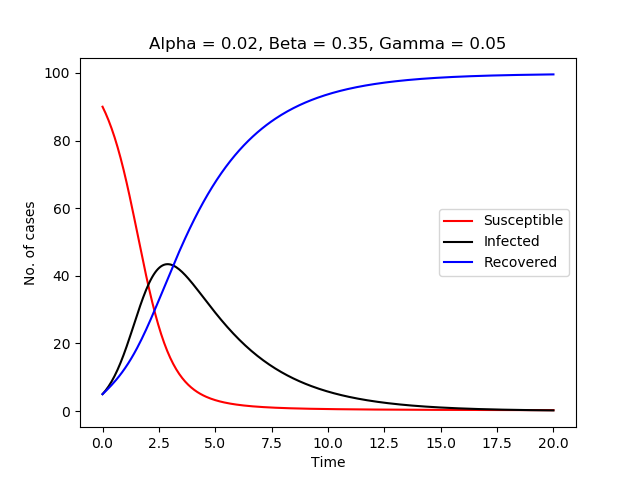
\includegraphics[scale=0.4]{fig/img/t_a2_b35_g5.png}\\
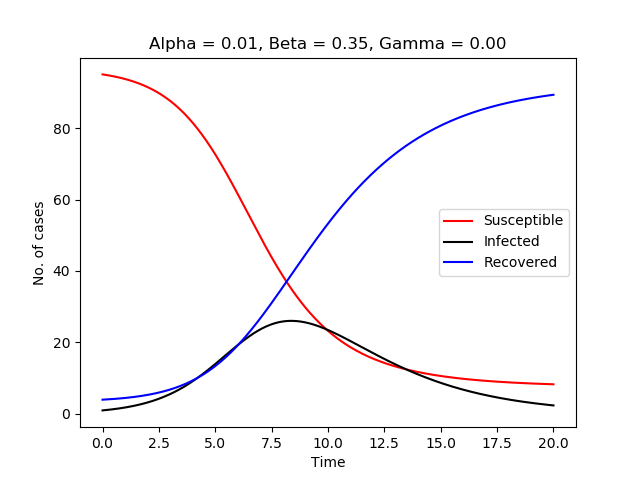
\includegraphics[scale=0.4]{fig/img/t_x1_1_x2_95.png}
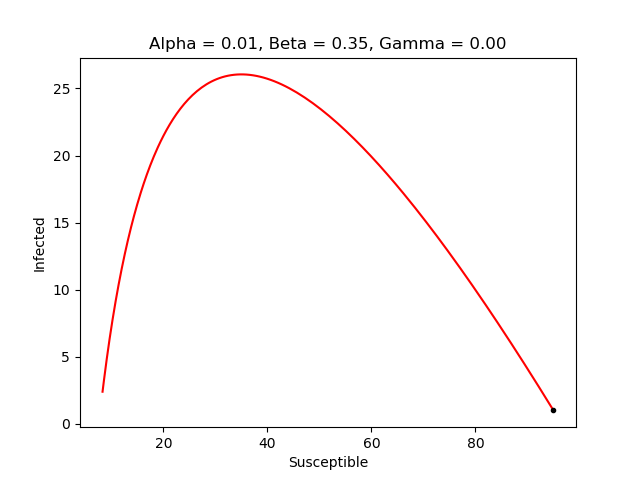
\includegraphics[scale=0.4]{fig/img/x1_1_x2_95.png}\\